\documentclass[11pt]{article}
\usepackage{matt}
\begin{document}

\section*{Update for the Week of \today}

\begin{figure}[h]
  \centering
  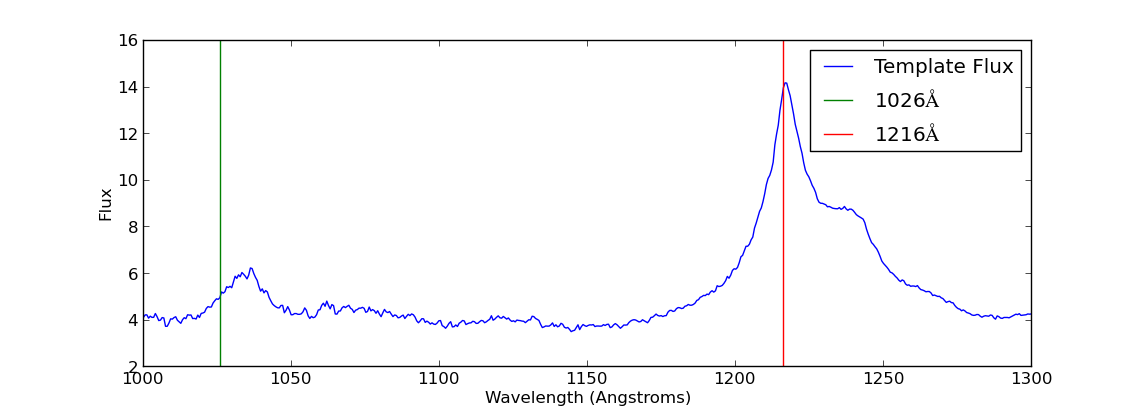
\includegraphics[width=15cm]{QSOTemplateCheck.png}
  \caption{The above figure shows the quasar template from {\tt LBQS.lis}. We also show the \lya\ line and the \lyb\ line. The emission line at $\sim 1070$\AA\ does not appear to match up with the \lyb\ line.}
  \label{fig:todo}
\end{figure}

\begin{figure}[h]
  \centering
  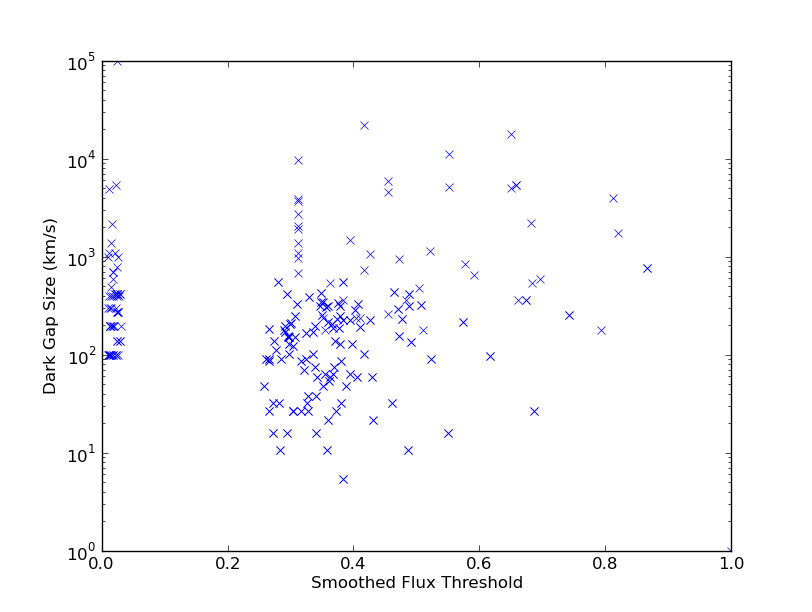
\includegraphics[width=8cm]{LvsT.png}
  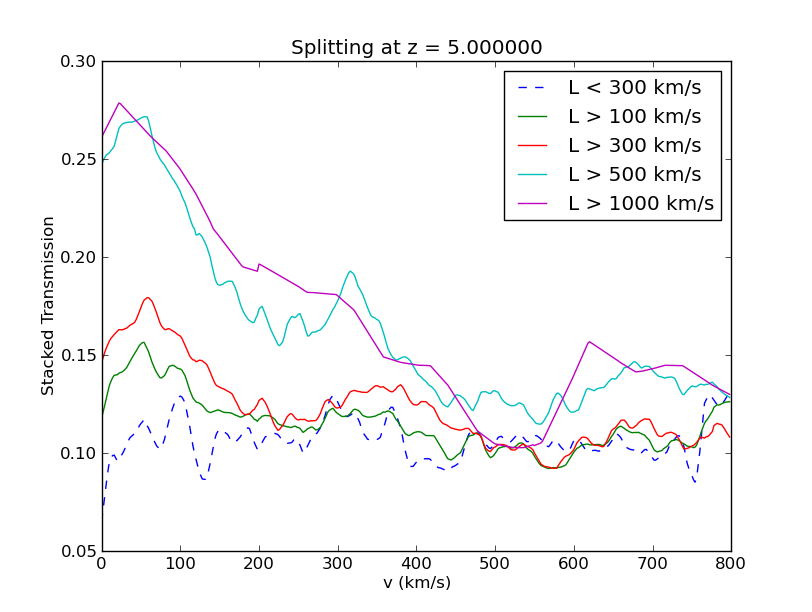
\includegraphics[width=8cm]{Stack_Zgreaterthan5.png}
  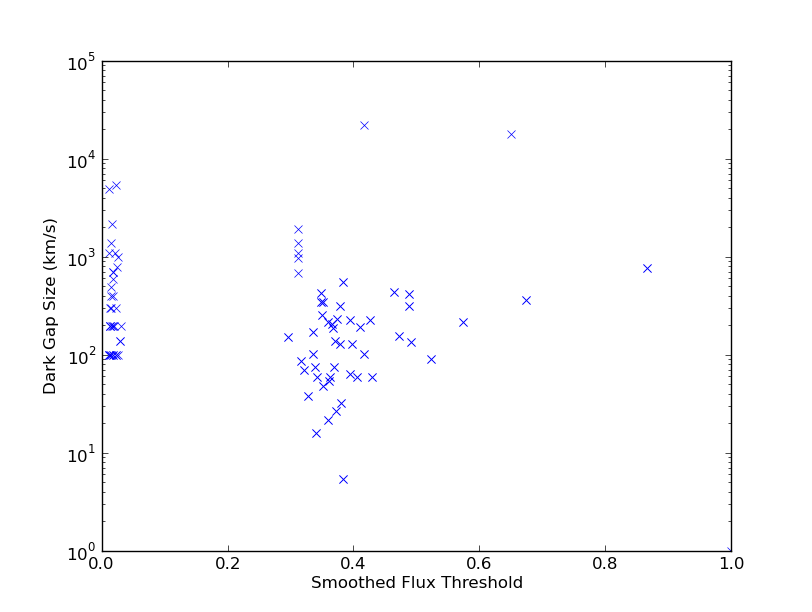
\includegraphics[width=8cm]{LvsT_zGreaterThan5p5.png}
  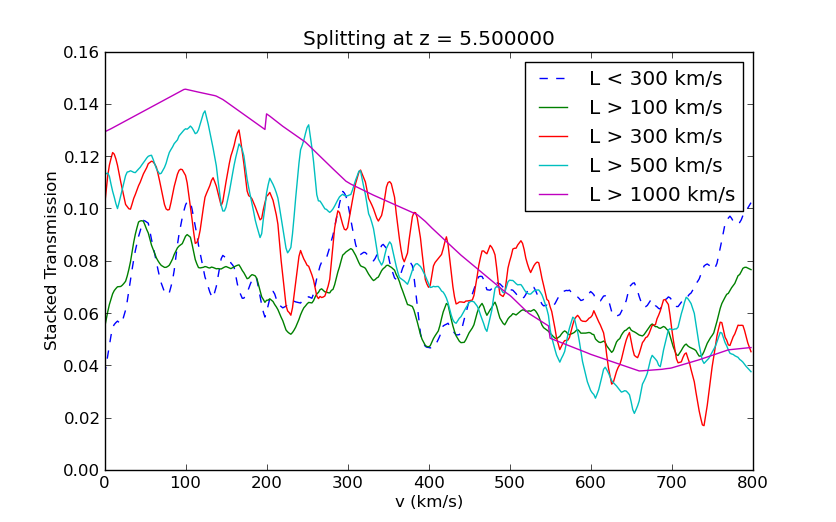
\includegraphics[width=8cm]{Stack_Zgreaterthan5p5.png}
  \caption{The left-hand plots here show a scatter plot of dark gap sizes along with the smoothed flux threshold below which a region can be identified as a dark gap. The right-hand plot shows the stacked transmission outside of dark gaps of varying lengths. The top row is for $z > 5$ and the bottom row is for $z > 5.5$. The point of these plots was to investigate why stacked transmission outside of large gaps appears to be larger than that outside of small gaps and I thought it might be a selection effect from noisy spectra having larger gaps and also larger thresholds for transmission to not count as saturated absorption.}
  \label{fig:todo}
\end{figure}


\begin{figure}[h]
  \centering
  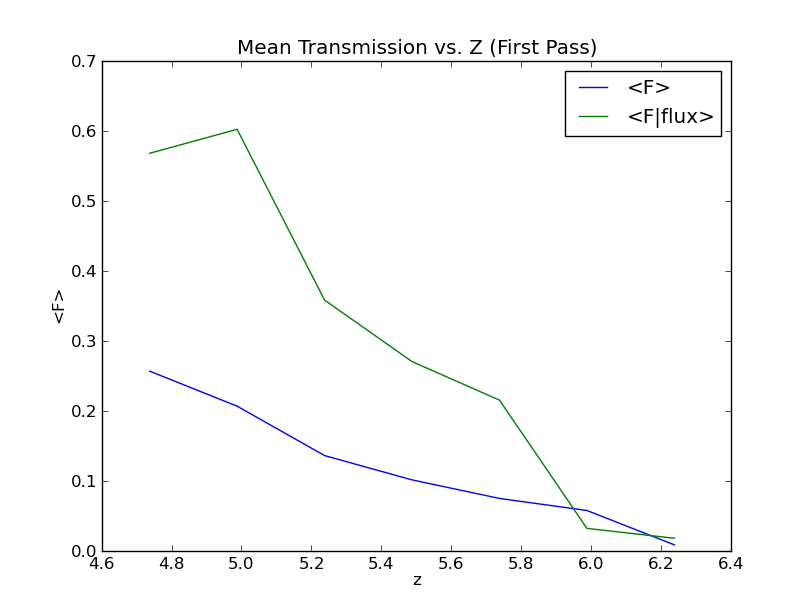
\includegraphics[width=8cm]{meanFs.png}
  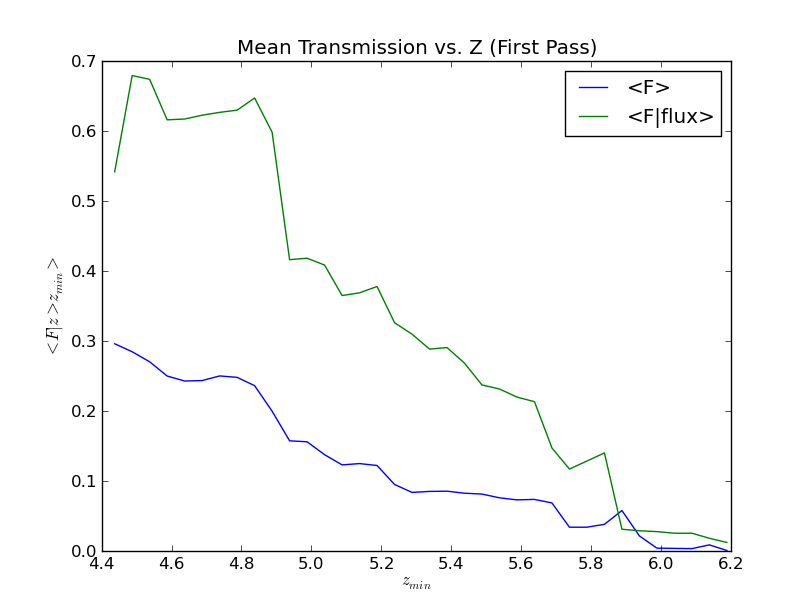
\includegraphics[width=8cm]{FluxCDF.png}
  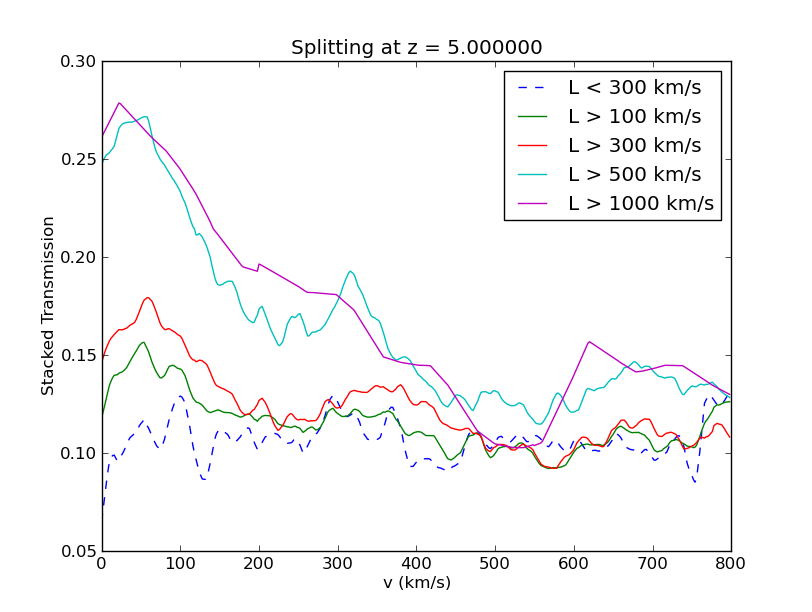
\includegraphics[width=8cm]{Stack_Zgreaterthan5.png}
  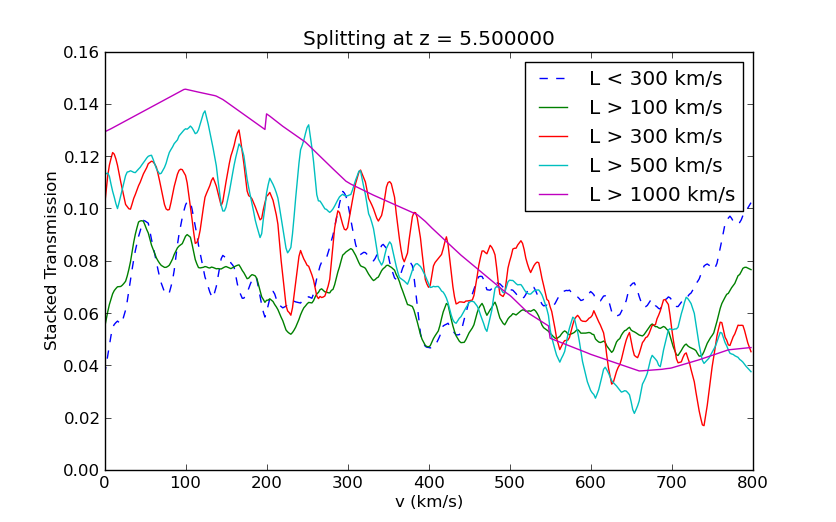
\includegraphics[width=8cm]{Stack_Zgreaterthan5p5.png}
  \caption{The top row shows two measures of the mean transmitted flux as a function of redshift. In the upper left-hand plot, we show $\langle F \rangle(z)$ (blue) and $\langle F | F > 0 \rangle(z)$ (green). In the upper right-hand plot we show $\langle F \rangle(z>z_{\text{min}})$ (blue) and $\langle F | F > 0 \rangle(z>z_{\text{min}})$. \textit{To be precise}, we aren't actually plotting $\langle F | F > 0\rangle$ but, instead, we are plotting the mean transmission in regions which are \textit{not identified as dark gaps}. In other words: $\langle F | \tilde{F} > 2\tilde{\sigma}_{N}\rangle$. In the bottom panels we show the \lya\ stacks for $z > 5$ (left) and $z > 5.5$ (right). }
  \label{fig:todo}
\end{figure}

\begin{figure}[h]
  \centering
  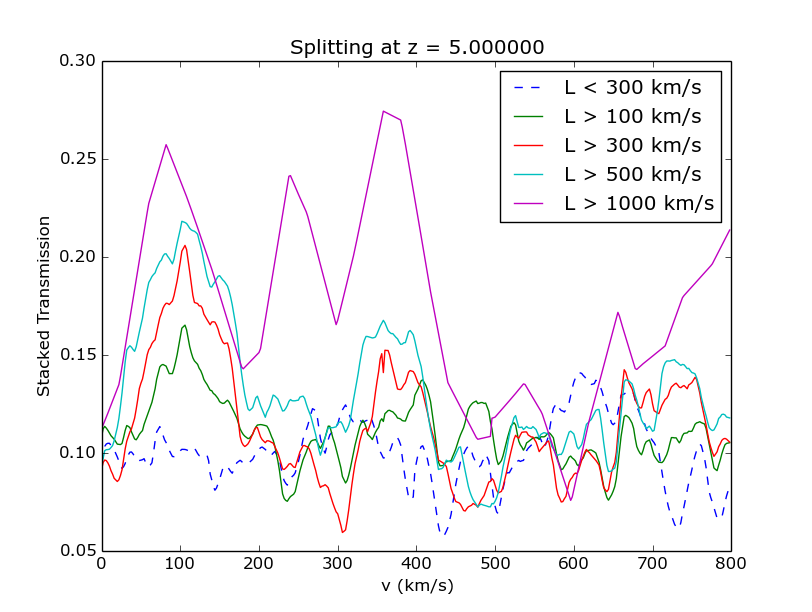
\includegraphics[width=8cm]{LybStack_zGreaterThan5.png}
  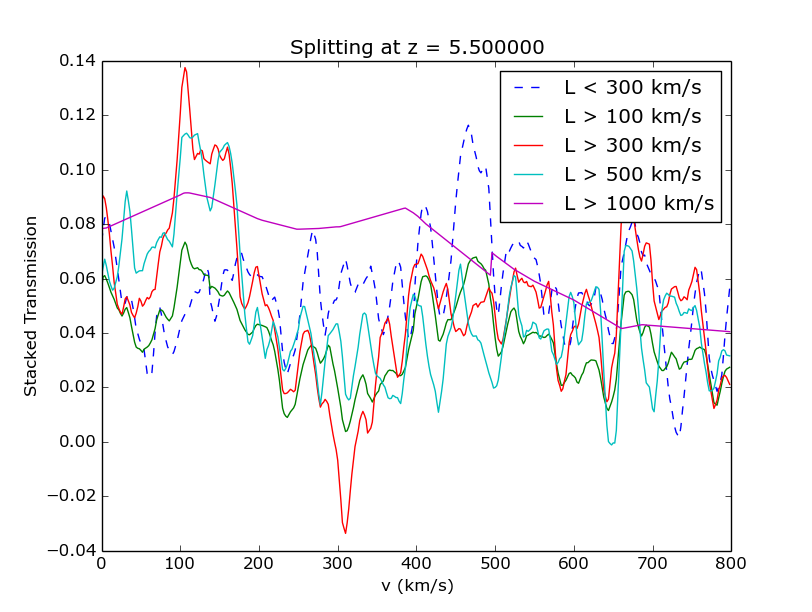
\includegraphics[width=8cm]{LybStack_zGreaterThan5p5.png}
  \caption{The above plots show the stacked \lya\ transmission outside of dark gaps \textit{in \lyb\ } of various sizes. The left-hand plot only includes dark gaps with $z_{\text{gap}} > 5$ and the right-hand plot only includes dark gaps with $z_{\text{gap}} > 5.5$.}
  \label{fig:todo}
\end{figure}

\begin{figure}[h]
  \centering
  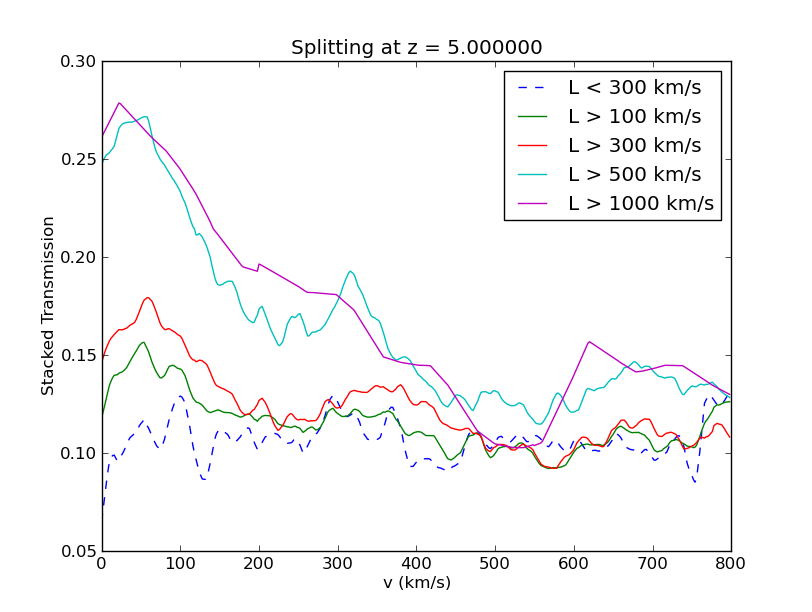
\includegraphics[width=8cm]{Stack_Zgreaterthan5.png}
  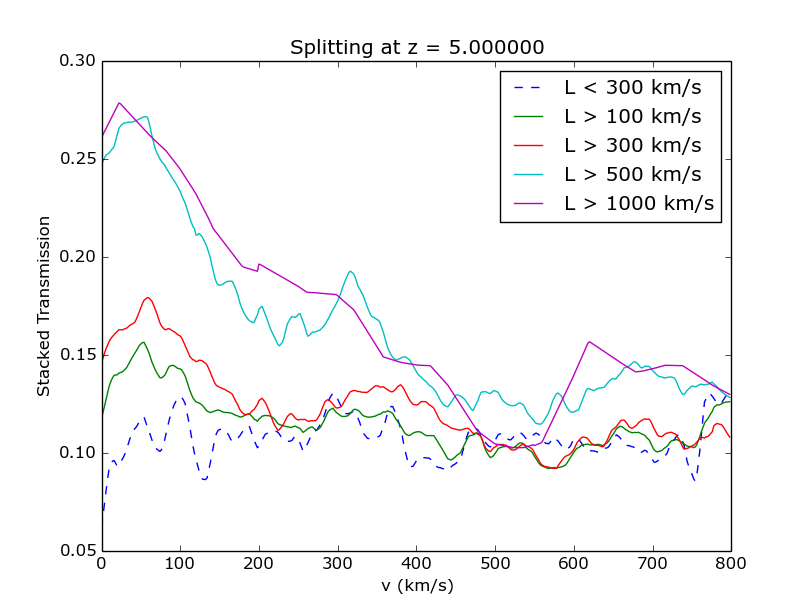
\includegraphics[width=8cm]{LybSanity_zGreaterThan5.png}
  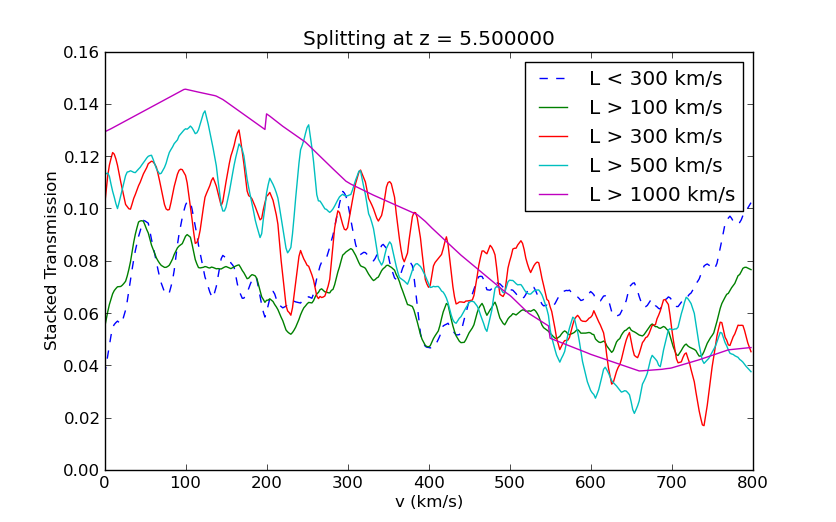
\includegraphics[width=8cm]{Stack_Zgreaterthan5p5.png}
  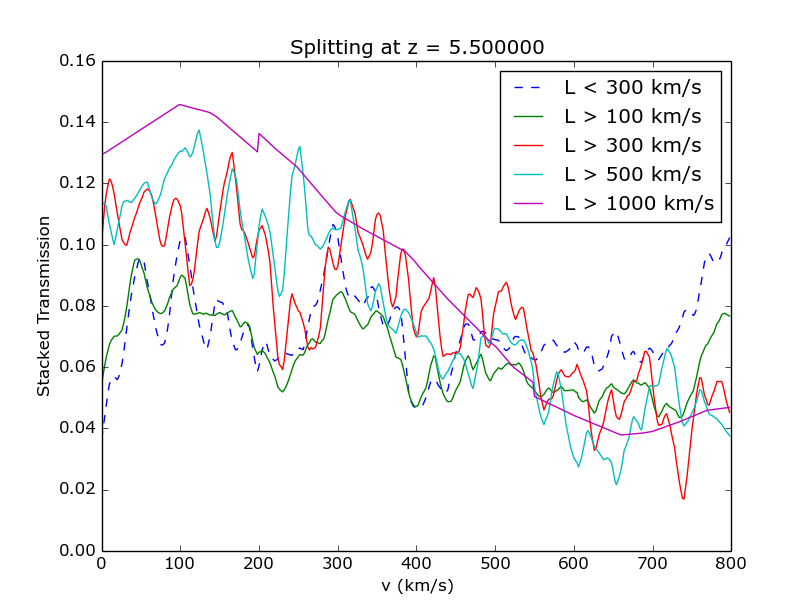
\includegraphics[width=8cm]{LybSanity_zGreaterThan5p5.png}
  \caption{The panels in each row should \textit{probably} be the same. This is a sanity check of the \lyb\ stacking code.}
  \label{fig:todo}
\end{figure}

\begin{figure}[h]
  \centering
  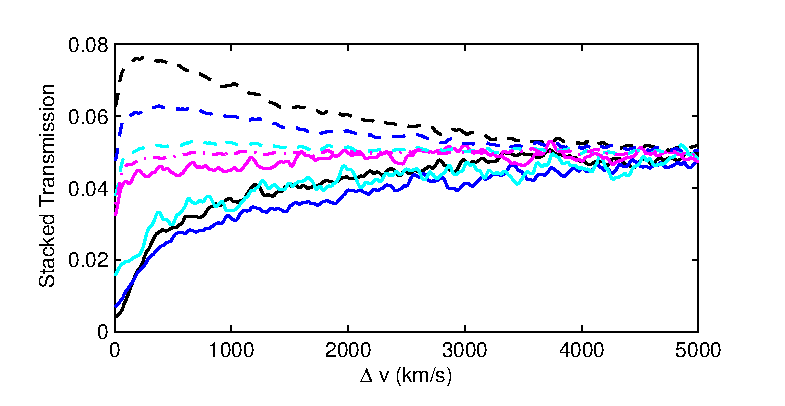
\includegraphics[width=14cm]{fig7a.eps}
  \caption{This figure is taken from our neutral islands paper and shows the expected stacked \lya\ transmission outside of large (solid) and small (dashed) dark gaps \textit{in \lyb}. }
  \label{fig:todo}
\end{figure}

\begin{figure}[h]
  \centering
  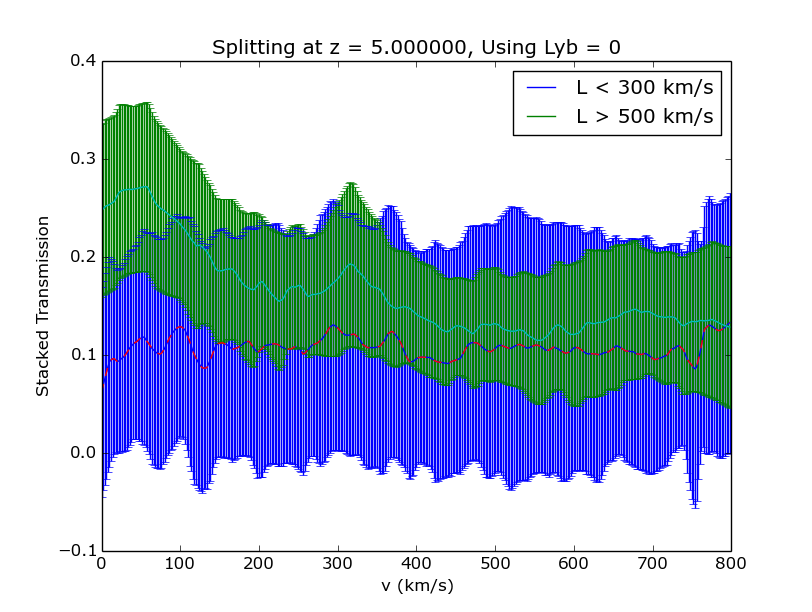
\includegraphics[width=8cm]{LyaStack_wErrors_500kms.png}
  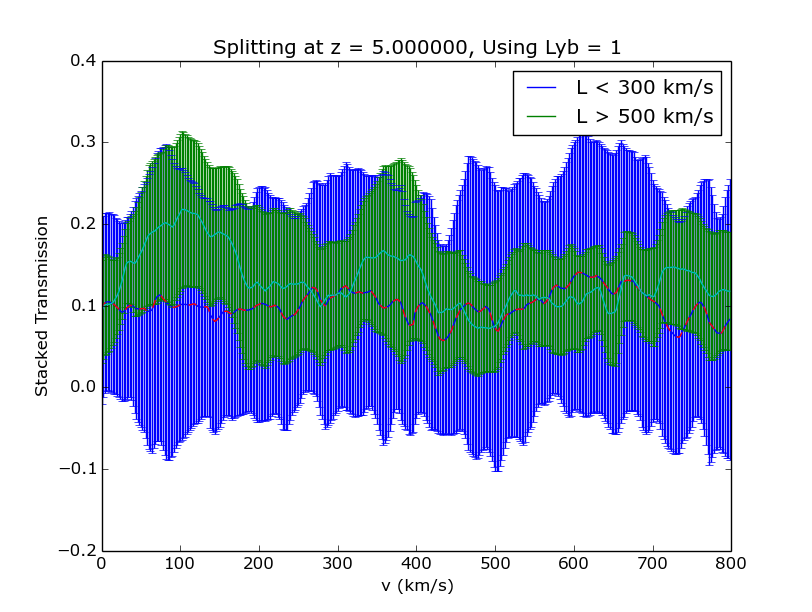
\includegraphics[width=8cm]{LybStack_wErrors_500kms.png}
  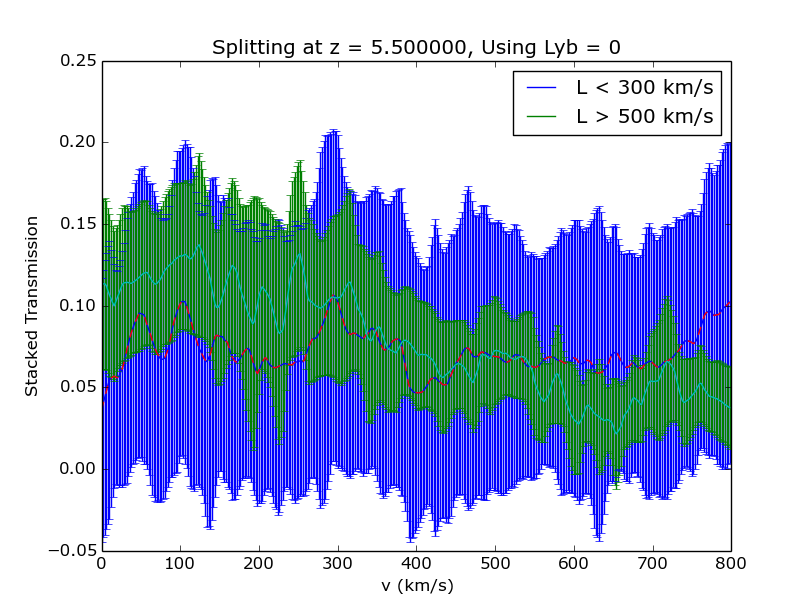
\includegraphics[width=8cm]{LyaStack_wErrors_500kms_z5p5.png}
  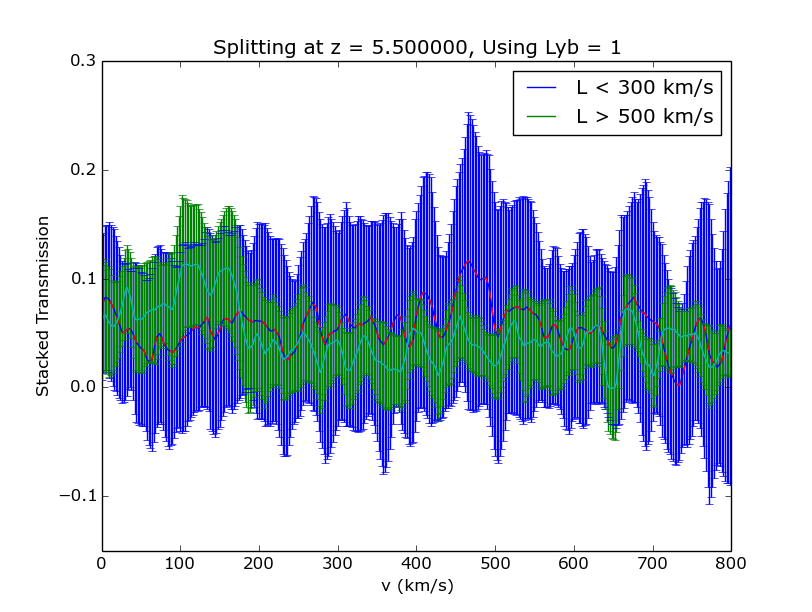
\includegraphics[width=8cm]{LybStack_wErrors_500kms_z5p5.png}
  \caption{The above panels show the effect of determining stacking locations according to dark gaps in \lyb\ spectra. The left-hand panels do \textit{not} stack according to \lyb\ dark gaps while the right-hand plots do. The top row only considers dark gaps with $z_{\text{gap}} > 5$ while the bottom row only considers gaps with $z_{\text{gap}} > 5.5$.}
  \label{fig:LybEffect}
\end{figure}

\begin{figure}[h]
  \centering
  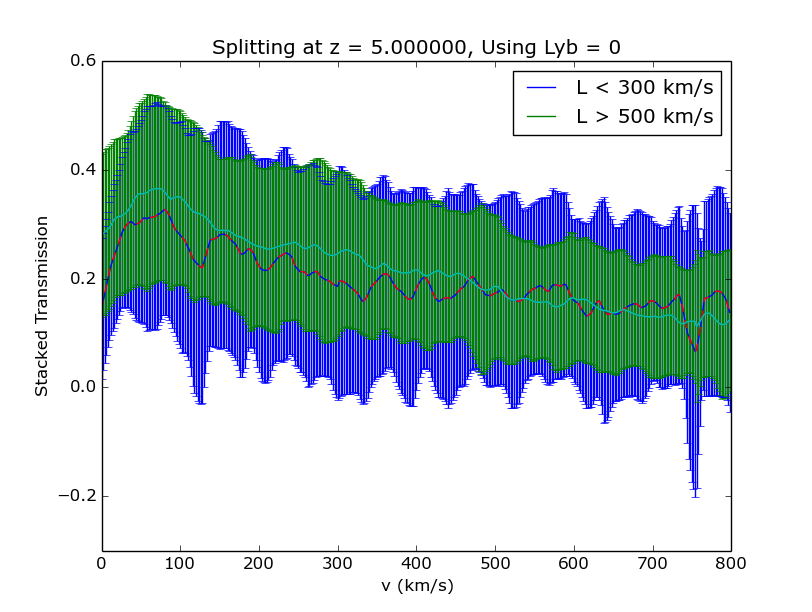
\includegraphics[width=8cm]{LyaStack_wErrors_500kms_z5_PLfit.png}
  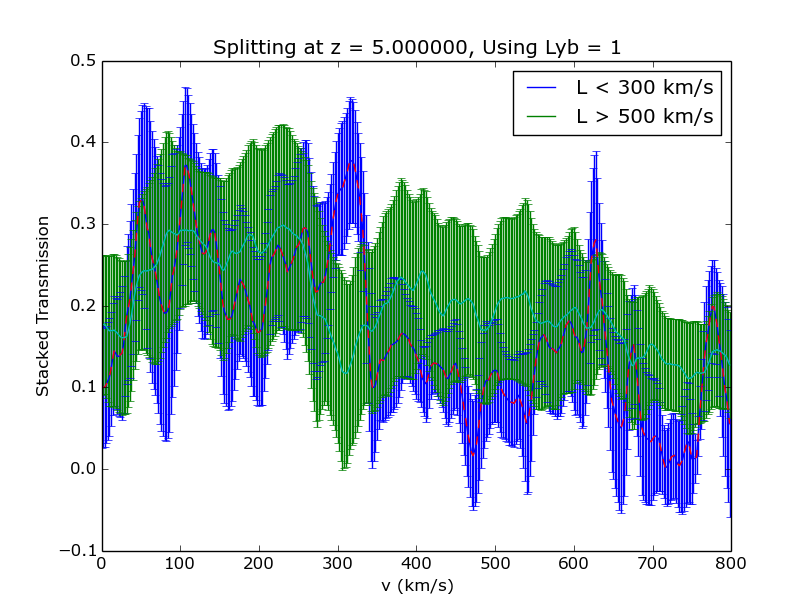
\includegraphics[width=8cm]{LybStack_wErrors_500kms_z5_PLfit.png}
  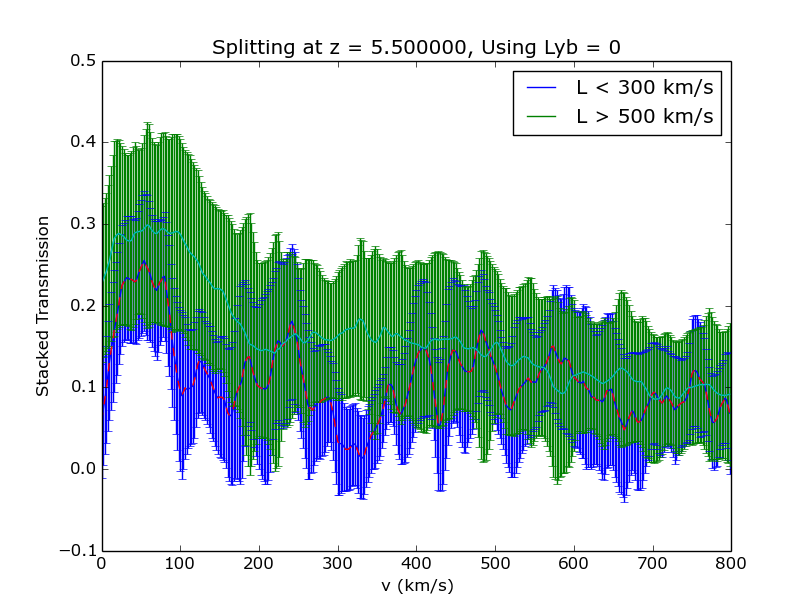
\includegraphics[width=8cm]{LyaStack_wErrors_500kms_z5p5_PLfit.png}
  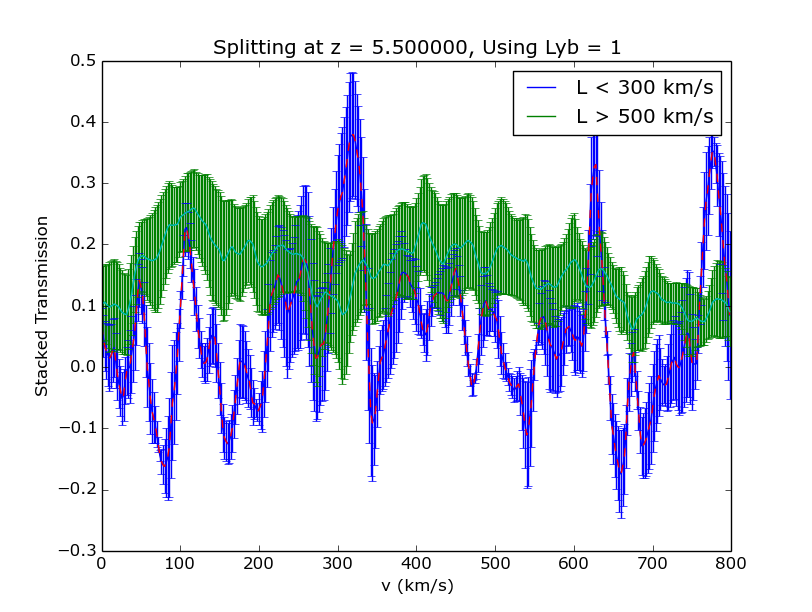
\includegraphics[width=8cm]{LybStack_wErrors_500kms_z5p5_PLfit.png}
  \caption{The above panels are identical to those in Fig. \ref{fig:LybEffect}, except that we have use a power law to fit the quasar continua: $F(\lambda) = F(\lambda_{R})\left(\lambda/\lambda_{R}\right)^{-1.56}$, where $\lambda_{R}$ is redward of \lya and $F_{R}$ is the average flux around this wavelength.}
  \label{fig:todo}
\end{figure}





\end{document}